%!TEX root = ../3dbook.tex
% chktex-file 46
% chktex-file 36

\setchapterpreamble[u]{\margintoc}

\graphicspath{{dtvd3d/}}
% \renewcommand*{\thelesson}{3.1}

\newcommand{\Orient}{O\textsc{rient}\xspace}
\newcommand{\Insphere}{I\textsc{n}S\textsc{phere}\xspace}

\chapter[Tetrahedralisations and 3D Voronoi diagrams]{Tetrahedralisations and \\3D Voronoi diagrams}%
\label{chap:dtvd3d}


The Delaunay triangulation (DT) and the Voronoi diagram (VD) are fundamental data structures when dealing with spatial datasets, many computer scientists and mathematicians consider the VD as being the most fundamental spatial structure (or spatial model) because it is very simple, and yet is so powerful that it helps in solving many theoretical problems, as well as many real-world applications.

The DT and the VD are most often presented, described, and used, in two dimensions, but their concepts can be generalised to higher dimensions.
We describe in this chapter the concepts in $\mathbb{R}^{3}$, and also discuss the $n$-dimensional cases when appropriate.%
\index{Euclidean space}\marginnote{three-dimensional Euclidean space}

We also discuss how the constrained and conforming DT can be generalised to $\mathbb{R}^{3}$.

\begin{kaobox}[frametitle=\faExternalLink\ To read or to watch.]
  The reader is advised to first read the Chapter \emph{Triangulations \& Voronoi diagram} in the book \emph{Computational modelling of terrains}~\citep{terrain_book}, where the 2D concepts are introduced.
\end{kaobox}

%%%
%
\section[3D Voronoi diagram]{The three-dimensional Voronoi Diagram}

Let $S$ be a set of points in $\mathbb{R}^d$. 
The Voronoi cell of a point $p \in S$, defined $\mathcal{V}_{p}$, is the set of points $x \in \mathbb{R}^d$ that are closer to $p$ than to any other point in $S$; that is:
\begin{equation}
\mathcal{V}_p = \{x \in \mathbb{R}^{d} \ | \ \|x-p\| \, \leq \, \|x-q\|, \ \forall \, q \in S \} 
\end{equation}
The union of the Voronoi cells of all generating points $p \in S$ form the Voronoi diagram of $S$, defined VD($S$). 
If $S$ contains only two points $p$ and $q$, then VD($S$) is formed by a single hyperplane defined by all the points $x \in \mathbb{R}^d$ that are equidistant from $p$ and $q$. 
This hyperplane is the perpendicular bisector of the line segment from $p$ to $q$, and splits the space into two (open) half-spaces. 
\index{half-space}
$\mathcal{V}_p$ is formed by the half-space containing $p$, and $\mathcal{V}_q$ by the one containing $q$. 

%

As shown in Figure~\ref{fig:halfspaces}, 
\begin{marginfigure}
  \centering
  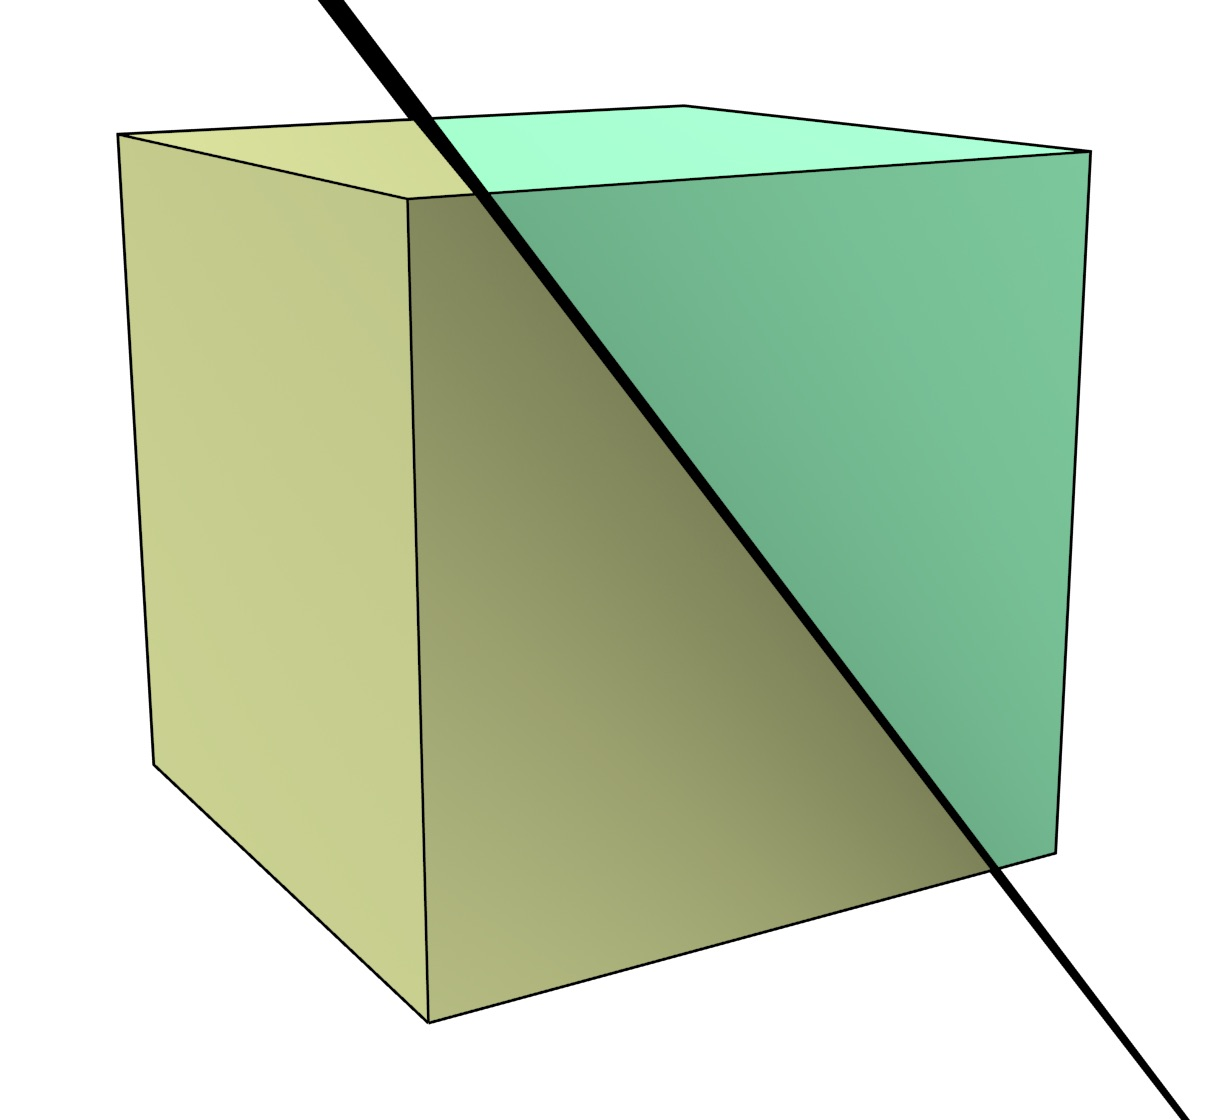
\includegraphics[width=0.8\textwidth]{figs/halfspaces}
  \caption[A Voronoi cell]{The Voronoi cell $\mathcal{V}_p$ is formed by the intersection of all the half-planes between $p$ and the other points.}%
\label{fig:halfspaces}
\end{marginfigure}
when $S$ contains more than two points (let us say it contains $n$ points), the Voronoi cell of a given point $p \in S$ is obtained by the intersection of $n-1$ half-spaces defined by $p$ and the other points $q \in S$. 
That means that $\mathcal{V}_{p}$ is always convex, in any dimensions. Notice also that every point $x \in \mathbb{R}^d$ has at least one nearest point in $S$, which means that VD($S$) covers the entire space.

%

As shown in Figures~\ref{fig:vd2d}, 
\begin{marginfigure}
  \centering
  \includegraphics[width=0.8\textwidth]{figs/vd2d}
  \caption[The VD for a set of points in the plane]{The VD for a set $S$ of points in the plane (the black points).}%
\label{fig:vd2d}
\end{marginfigure}
the VD of a set $S$ of points in $\mathbb{R}^2$ is a planar graph, but it can also be seen as a two-dimensional cell complex where each 2-cell is a (convex) polygon. 
Two Voronoi cells, $\mathcal{V}_{p}$ and $\mathcal{V}_{q}$, lie on the opposite sides of the perpendicular bisector separating the points $p$ and $q$. 

%

In $\mathbb{R}^3$, VD($S$) is a three-dimensional cell complex. 
The Voronoi cell of a point $p$ is formed by the intersection of all the half-spaces (three-dimensional planes) between $p$ and the other points in $S$. 
Drawing a picture of the three-dimensional case is not easy, thus Figure~\ref{fig:vd3d} shows two adjacent Voronoi cells (which are convex polyhedra), and Figure~\ref{fig:vd3d_onecell} one cell with its incident Delaunay edges.
\begin{marginfigure}
  \centering
  \includegraphics[width=0.8\textwidth]{figs/vd3d}
  \caption[Two Voronoi cells adjacent to each other]{Two Voronoi cells adjacent to each other in $\mathbb{R}^3$, they share the grey face.}%
\label{fig:vd3d}
\end{marginfigure}
\begin{marginfigure}
  \centering
  \includegraphics[width=\textwidth]{figs/vd3d_onecell}
  \caption[The Voronoi cell for a vertex]{The Voronoi cell for the red vertex, the red edges are the Delaunay edges that are dual to the Voronoi facets.}%
\label{fig:vd3d_onecell}
\end{marginfigure}

%

The VD has many properties, and most of them are valid in any dimensions. 
Note that most of these properties are valid only when the set $S$ of points is in \emph{general position}, that is when for example in three dimensions no five points are cospherical, and no four points are collinear. 
Details concerning the possible degeneracies are given in Section~\ref{sec:degeneracies}. 
What follows is a list of the most relevant properties:
\begin{description}
  \item[Size:] if $S$ has $n$ points, then VD($S$) has exactly $n$ Voronoi cells since there is a one-to-one mapping between the points and the cells.
  \item[Voronoi vertices:] in $\mathbb{R}^d$, a Voronoi vertex is equidistant from ($d+1$) points. In $\mathbb{R}^3$, a Voronoi vertex is at the centre of a sphere defined by 4 points in $S$.
  \item[Voronoi edges:] in $\mathbb{R}^d$, a Voronoi edge is equidistant from $d$ points.
  \item[Voronoi faces:] in $\mathbb{R}^d$, a Voronoi face is equidistant from ($d-1$) points. Hence, in $\mathbb{R}^3$, it is the bisector plane perpendicular to the line segment joining two points.
  \item[Convex hull:] let $S$ be a set of points in $\mathbb{R}^d$, and $p$ one of its points. $\mathcal{V}_{p}$ is unbounded if $p$ bounds conv($S$). Otherwise, $\mathcal{V}_{p}$ is the convex hull of its Voronoi vertices. 
\end{description}


%%%
%
\section[Delaunay tetrahedralisation]{The Delaunay tetrahedralisation}

The Delaunay triangulation of a set $S$ of points in $\mathbb{R}^d$ is a simplicial complex where each $d$-simplex $\sigma$, formed by $d+1$ vertices in $S$, has an empty \emph{circumball} (a ball is said to be \emph{empty} when no points are in its interior). 
\begin{marginfigure}
  \centering
  \includegraphics[width=\textwidth]{figs/dt2d_2}
  \caption{The DT of a set of points in the plane.}%
  \label{fig:dt2d_2}
\end{marginfigure}
For $\mathbb{R}^3$, it is called the \emph{Delaunay tetrahedralisation}: the space is tessellation into non-overlapping tetrahedra having an empty \emph{circumsphere} (as shown in Figure~\ref{fig:dt3d}).
\begin{marginfigure}
  \centering
  \includegraphics[width=0.8\textwidth]{figs/dt3d}
  \caption{A Delaunay tetrahedron has an empty circumsphere.}%
\label{fig:dt3d}
\end{marginfigure}


%%%
\subsection{Duality between the DT and the VD}

The VD and the DT are dual to each other, and that in any dimensions.
This means they represent the same thing but from a different point-of-view, and one structure can always be extracted from the other.
Consider a graph embedded in $\mathbb{R}^{d}$ as a $d$-dimensional cell complex. 
The mappings between the elements of a cell complex in $\mathbb{R}^{d}$ are as follows: let $C$ be a $k$-cell, the dual cell of $C$ in $\mathbb{R}^{d}$ is denoted by $C^{\star}$ and is a ($d-k$)-cell. 

%

The duality between the VD and the DT in $\mathbb{R}^3$ are thus as follows: 
\begin{figure}
  \centering
  \includegraphics[width=1.0\textwidth]{figs/duality_3d}
  \caption{Duality in $\mathbb{R}^{3}$ between the elements of the VD and the DT.}%
\label{fig:duality_3d}
\end{figure}
\begin{itemize}
  \item a Delaunay vertex $p$ becomes a Voronoi cell (Figure~\ref{fig:duality_3d}a); 
  \item a Delaunay edge $\alpha$ becomes a Voronoi face (Figure~\ref{fig:duality_3d}b);
  \item a Delaunay triangular face $\kappa$ becomes a Voronoi edge (Figure~\ref{fig:duality_3d}c);
  \item a Delaunay tetrahedron $\tau$ becomes a Voronoi vertex (Figure~\ref{fig:duality_3d}d). 
\end{itemize}
A Voronoi vertex is located at the centre of the sphere circumscribed to its dual tetrahedron, and two vertices in $S$ have a Delaunay edge connecting them if and only if their two respective dual Voronoi cells are adjacent.


%%%
\subsection{Convex Hull}
In any dimensions, the DT of set $S$ of points subdivides completely conv($S$), \ie\ the union of all the simplices in DT($S$) is conv($S$).
The boundary of a convex hull in 3D is formed of a set of triangles.
Figure~\ref{fig:dt2}b shows an example.
\begin{figure*}
  \centering
  \begin{subfigure}[b]{0.29\linewidth}
    \includegraphics[width=\textwidth]{figs/t1}
    \caption{}
  \end{subfigure}%
  \qquad
  \begin{subfigure}[b]{0.29\linewidth}
    \includegraphics[width=\textwidth]{figs/t2}
    \caption{}
  \end{subfigure}%
  \qquad
  \begin{subfigure}[b]{0.29\linewidth}
    \includegraphics[width=\textwidth]{figs/t3}
    \caption{}
  \end{subfigure}%
  \caption[A set of points, its convex hull and its Delaunay tetrahedralisation]{\textbf{(a)} A set of 1000 points randomly distributed in a cube. \textbf{(b)} Its convex hull. \textbf{(c)} The Delaunay tetrahedralisation of the points, `sliced' in the middle and the upper tetrahedra removed (to be able to visualise the interior).}%
\label{fig:dt2}
\end{figure*}


%%%
\subsection{Local Optimality}
Let $\mathcal{T}$ be a triangulation of $S$ in $\mathbb{R}^d$. 
A facet $\sigma$ 
\index{facet}\marginnote{facet}
(a ($d-1$)-simplex) is said to be \emph{locally} Delaunay if it either:
\begin{description}
  \item[(i)] belongs to only one $d$-simplex, and thus bounds conv($S$), or
  \item[(ii)] belongs to two $d$-simplices $\sigma_a$ and $\sigma_b$, formed by the vertices of $\sigma$ and respectively the vertices $a$ and $b$, and $b$ is outside of the circumball of $\sigma_a$.
\end{description}
The second case is illustrated in two dimensions in Figure~\ref{fig:slivers}a. 
\begin{figure}
  \centering
  \includegraphics[width=0.9\textwidth]{figs/slivers}
  \caption[A four-sided convex polygon can be triangulated in two different ways]{\textbf{(a)} A four-sided convex polygon $abcd$ can be triangulated in two different ways, but the empty circumcircle criterion guarantees that the triangles are as equilateral as possible. Notice that the edge $ac$ is not locally Delaunay, but $bd$ is. \textbf{(b)} In three dimensions, five vertices can be triangulated with either two or three tetrahedra. Although the tetrahedralisation at the bottom has two nicely shaped tetrahedra, they are not Delaunay (the point $d$ is inside the sphere $abce$, which also implies that $b$ is inside the sphere $acde$). The tetrahedralisation at the top respects the Delaunay criterion, but contains one very thin tetrahedron spanned by the points $a$, $b$, $d$ and $e$.}%
\label{fig:slivers}
\end{figure}
In an arbitrary triangulation, not every facet that is locally Delaunay is necessarily a facet of DT($S$), but local optimality implies globally optimality in the case of the DT:
\begin{quote}
  Let $\mathcal{T}$ be a triangulation of a point set $S$ in $\mathbb{R}^d$. If every facet of $\mathcal{T}$ is locally Delaunay, then $\mathcal{T}$ is the Delaunay triangulation of $S$.
  \marginnote{locally Delaunay}
\end{quote}
This has serious implications as the DT---and its dual---are locally modifiable, \ie\ we can theoretically insert, delete or move a points in $S$ without recomputing DT($S$) from scratch.


%%%
\subsection{Angle Optimality}
The DT in two dimensions has a very important property that is useful in applications such as finite element meshing or interpolation: the \emph{max-min angle optimality}.
\marginnote{max-min angle optimality}\index{max-min angle optimality}
Among all the possible triangulations of a set $S$ of points in $\mathbb{R}^2$, DT($S$) maximises the minimum angle (max-min property), and also minimises the maximum circumradii. 
In other words, it creates triangles that are as equilateral as possible. 

%

Finding `good' tetrahedra, \ie\ nicely shaped, is however more difficult than finding good triangles because the max-min property of Delaunay triangles does not generalise to three dimensions. 
A DT in $\mathbb{R}^3$ can indeed contain some tetrahedra, called \emph{slivers}, 
\marginnote{slivers}\index{slivers}
whose four vertices are almost coplanar (see Figure~\ref{fig:slivers}b); these tetrahedra are Delaunay. 
Note that such slivers do not have two-dimensional counterparts.

%

For many applications where the Delaunay tetrahedralisation is used, \eg\ in the finite element method in engineering or when the tetrahedra are used to perform interpolation directly, these tetrahedra are bad and must be removed. 
Why use the DT in three dimensions then?
First, it should be said that in most cases Delaunay tetrahedra have in general a more desirable shape than arbitrary tetrahedra, they tend to favour `round' tetrahedra. 
Second, the VD is not affected by them: Voronoi cells in three dimensions will still be `relatively spherical' even if the DT has many slivers. 
Third, if the VD is used for interpolation, then the VD is necessary because many GIS operations use the properties of the VD (see Section~\ref{sec:interpol}), and if only one tetrahedron does not have an empty circumsphere, then the VD is corrupted.



%%%
\subsection{Lifting on the paraboloid}%
\label{sec:parabolic_lifting}

There exists a close relationship between DTs in $\mathbb{R}^{d}$ and convex polytopes in $\mathbb{R}^{d+1}$. 

Let $S$ be a set of points in $\mathbb{R}^{d}$, and let $x_{1}, x_{2}, \ldots , x_{d}$ be the coordinates axes. 
The parabolic lifting map projects each vertex $v(v_{x1}, v_{x2}, \ldots , v_{xd})$ to a vertex $v^{+}(v_{x1}, v_{x2}, \ldots , v_{xd}, v_{x1}^{2}+v_{x2}^{2}+\cdots+v_{xd}^{2})$ on the paraboloid of revolution in $\mathbb{R}^{d+1}$. 
The set of points thus obtained is denoted $S^{+}$. 
Observe that, for the two-dimensional case, the paraboloid in three dimensions defines a surface whose vertical cross sections are parabolas, and whose horizontal cross sections are circles; the same ideas are valid in higher dimensions. 

%

The relationship is the following: every facet (a $d$-dimensional simplex) of the lower envelope of conv($S^{+}$) projects to a $d$-simplex of the Delaunay triangulation of $S$. 
This is illustrated in Figure~\ref{fig:paraboloid} for the construction of the DT in $\mathbb{R}^{2}$. 
\begin{marginfigure}
  \centering
  \includegraphics[width=0.95\textwidth]{figs/paraboloid}
  \caption{The parabolic lifting map for a set $S$ of points $\mathbb{R}^2$.}%
\label{fig:paraboloid}
\end{marginfigure}

%

In short, the construction of the $d$-dimensional DT can be transformed into the construction of the convex hull of the lifted set of points in ($d+1$) dimensions.
In practice, since it is easier to construct convex hulls (especially in higher dimensions, \ie\ 4+), the DT is often constructed with this method.


%%%
\subsection{Degeneracies}%
\label{sec:degeneracies}

The previous definitions of the VD and the DT assumed that the set $S$ of points is in general position, \ie\ the distribution of points does not create any ambiguity in the two structures. 
For the VD/DT in $\mathbb{R}^{d}$, the degeneracies, or special cases, occur when $d+1$ points lie on the same hyperplane and/or when $d+2$ points lie on the same ball. 
For example, in three dimensions, when five or more points in $S$ are cospherical there is an ambiguity in the definition of DT($S$). 
This implies that DT($S$) is not unique; VD($S$) is still unique, but it has different properties.


%%%
%
\section[Construction of 3D DT/VD]{Construction of the 3D DT/VD}

As is the case in 2D, there exist several algorithms to construct either the DT or the VD from a set of points in 3D.

%

Mainly three paradigms of computational geometry can be used for computing a Delaunay triangulation in two and three dimensions:  divide-and-conquer, sweep plane, and incremental insertion.
In two dimensions, each one of these paradigms yields an optimal algorithm.
In three dimensions, things are a bit more complicated.
Divide-and-conquer algorithms have a worst time complexity of $\mathcal{O}(n^3)$, although in practice they are subquadratic.
Only incremental insertion algorithms have a complexity that is worst-case optimal, \ie\ $\mathcal{O}(n^2)$ since the complexity of the DT in $\mathbb{R}^3$ is quadratic.
That is, there are configurations of $n$ points that yield a DT with $\mathcal{O}(n^2)$ tetrahedra.

%

And as is the case in 2D, it is often simpler to reconstruct and store the DT (because they have only 4 vertices and 4 neighbours) and to extract the VD on-the-fly when needed.

%

The details of the algorithms are out of scope for this course.
We provide in the following a general idea of how the reconstruction of the DT is performed in 3D by generalising the algorithm described in GEO1015.

\begin{kaobox}[frametitle=\faCog\ How does it work in practice?]
  Even more than in 2D, the duality between the convex hull in $d+1$-dimension and the DT in $d$-dimension is in practice exploited.
  Indeed, one can construct the convex hull of a set of points projected to 4D to obtain the DT in 3D.
  One popular and widely used implementation is Qhull (\url{http://www.qhull.org/}).
\end{kaobox}


%%%
\subsection{Generalisation of the flip-based incremental insertion algorithm}

The algorithm described in Algorithm~\ref{algo:insert1pt} is a generalisation to 3D of the flip-based incremental insertion algorithm used for 2D DT\@.
\begin{algorithm}[tb] 
  \DontPrintSemicolon\
  \KwIn{A DT($S$) $\mathcal{T}$ in $\mathbb{R}^3$, and a new point $p$ to insert}
  \KwOut{$\mathcal{T}^{p} = \mathcal{T} \cup \{p\}$}
  find tetrahedron $\tau$ containing $p$\;
  insert $p$ in $\tau$ by splitting it in to 4 new tetrahedra (flip14)\;
  push 4 new tetrahedra on a stack\;
  \While{stack is non-empty}
  {
    $\tau = \{p,a,b,c\} \leftarrow$ pop from stack\;
    $\tau_{a} = \{a,b,c,d\} \leftarrow$ get adjacent tetrahedron of $\tau$ having the edge $abc$ as a face\;
    \If{$d$ is inside circumsphere of $\tau$}
    {
      \If{configuration of $\tau$ and $\tau_a$ allows it}
      {
        flip the tetrahedra $\tau$ and $\tau_{a}$ (flip23 or flip32)\;
        push 2 or 3 new tetrahedra on stack\;
      }
      \Else{Do nothing} 
    }
  }
  \caption{Algorithm to insert one point in a DT}%
\label{algo:insert1pt}
\end{algorithm} 

Most steps can be generalised in a direct way.
Figure~\ref{fig:insertion_steps} shows the steps from the 2D algorithm, which are conceptually the same for the 3D generalisation of the algorithm (and it is more difficult to draw these steps in 3D).
\begin{figure*}
  \centering
  \includegraphics[width=1.5\textwidth]{figs/insertion_steps}
  \caption[Step-by-step insertion of a single point in a DT in two dimensions]{Step-by-step insertion, with flips, of a single point in a DT in two dimensions.}%
\label{fig:insertion_steps}
\end{figure*}




As is the case with the two-dimensional algorithm, the point $p$ is first inserted in $\mathcal{T}$ with a flip (\emph{flip14} in the case here), 
\marginnote{flips}\index{flip14}
and the new tetrahedra created must be tested to make sure they are Delaunay. 
The sequence of flips needed is controlled by a stack containing all the tetrahedra that have not been tested yet. 
The stack starts with the four resulting tetrahedra of the \emph{flip14}, and each time a flip is performed, the new tetrahedra created are added to the stack. 
The algorithms stops when all the tetrahedra incident to $p$ are Delaunay, which also means that the stack is empty.


%%%
\paragraph{Initialisation: the big tetrahedron.}
A DT is initialised with a tetrahedron several times larger than the spatial extent of $S$.
The points in $S$ are therefore always added inside an existing tetrahedron. 

%%%
\paragraph{Walk/Point location.}
To find the tetrahedron containing the newly inserted point $p$, the adjacency relationships between the tetrahedra can be used. 
With a series of \Orient\ tests one can navigate from one tetrahedron to the other.

%%%
\paragraph{Flips.}
A flip is a local (topological) operation that modifies the configuration of some adjacent tetrahedra. 
In 2D, for 4 points, a flip (called \emph{flip22}), modifies the configuration of 2 adjacent triangles by flipping the diagonal of the quadrilateral.
In 3D, there are 2 kinds of flips: \emph{flip23} and \emph{flip32}.
Consider the set $S = \{a, b, c, d, e\}$ of points in general position in $\mathbb{R}^{3}$ and its convex hull conv($S$). 
There exist two possible configurations, as shown in Figure~\ref{fig:flips3d}:
\begin{marginfigure}
  \centering
  \includegraphics[width=\textwidth]{figs/flips3d}
  \caption{The 4 different kinds of flips in 3D.}% 
\label{fig:flips3d}
\end{marginfigure}
\begin{enumerate}
  \item the five points of $S$ lie on the boundary of conv($S$); see Figure~\ref{fig:flips3d}a. There are exactly two ways to tetrahedralise such a polyhedron: either with two or three tetrahedra. In the first case, the two tetrahedra share a triangular face $bcd$, and in the latter case the three tetrahedra all have a common edge $ae$.
  \item one point $e$ of $S$ does not lie on the boundary of conv($S$), thus conv($S$) forms a tetrahedron; see Figure~\ref{fig:flips3d}b. The only way to tetrahedralise $S$ is with four tetrahedra all incident to $e$.
\end{enumerate}
Based on these two configurations, four types of flips in $\mathbb{R}^{3}$ can be described: \emph{flip23}, \emph{flip32}, \emph{flip14} and \emph{flip41} (the numbers refer to the number of tetrahedra before and after the flip). 
When $S$ is in the first configuration, two types of flips are possible: a \emph{flip23} is the operation that transforms one tetrahedralisation of two tetrahedra into another one with three tetrahedra; and a \emph{flip32} is the inverse operation. 
If $S$ is tetrahedralised with two tetrahedra and the triangular face $bcd$ is not locally Delaunay, then a \emph{flip23} will create three tetrahedra whose faces are locally Delaunay. 

A \emph{flip14} refers to the operation of inserting a vertex inside a tetrahedron, and splitting it into four tetrahedra; and a \emph{flip41} is the inverse operation that deletes a vertex.

Flips can not always be applied during an insertion, it depends on the local configuration.
For example, in Figure~\ref{fig:flips3d}a, a \emph{flip23} is possible on the two adjacent tetrahedra $abcd$ and $bcde$ if and only if the line $ae$ passes through the triangular face $bcd$ (which also means that the union of $abcd$ and $bcde$ is a convex polyhedron). 
If not, then a \emph{flip32} is possible if and only if there exists in the tetrahedralisation a third tetrahedron adjacent to both $abcd$ and $bcde$.



%%%
\subsection{Predicates}

The `orientation' of points in three dimensions is somewhat tricky because, unlike in two dimensions, we can not simply rely on the counter-clockwise orientation. 
In three dimensions, the orientation is always relative to another point of reference, \ie\ given three points we cannot say if a fourth one is left of right, this depends on the orientation of the three points.
When dealing with a single tetrahedron $\tau$ formed by the four vertices $a$, $b$, $c$ and $d$ (as in Figure~\ref{fig:orient}), 
\begin{marginfigure}
  \centering
  \includegraphics[width=0.9\textwidth]{figs/orient}
  \caption[Orientation of a tetrahedron]{The tetrahedron $abcd$ is correctly oriented since \Orient($a,b,c,d$) returns a positive result. The arrow indicates the correct orientation for the face $\sigma_a$, so that \Orient($\sigma_a,a$) returns a positive result.}%
\label{fig:orient}
\end{marginfigure}
we say that $\tau$ is correctly oriented if \Orient($a,b,c,d$) returns a positive value. 
Notice that if two vertices are swapped in the order, then the result is the opposite (\ie\ \Orient($a,c,b,d$) returns a negative value). 

Vertices forming a face in a tetrahedron $\tau$ can also be ordered. 
As shown in Figure~\ref{fig:orient}, a face $\sigma_a$, formed by the vertices $b$, $c$ and $d$, is correctly oriented if \Orient($\sigma_a,a$) gives a positive result---in the case here, \Orient($b,c,d,a$) gives a negative result, therefore the correct orientation of $\sigma_a$ is $cbd$. Observe that the face $bcd$ is called $\sigma_a$ because it is `mapped' to the vertex $a$ that is opposite; each of the four faces of a tetrahedron can be referred to in this way.

\Orient\ determines if a point $p$ is over, under or lies on a plane defined by three points $a$, $b$ and $c$.
It returns a positive value when the point $p$ is above the plane defined by $a$, $b$ and $c$; a negative value if $p$ is under the plane; and exactly 0 if $p$ is directly on the plane.
\Orient\ is consistent with the left-hand rule: when the ordering of $a$, $b$ and $c$ follows the direction of rotation of the curled fingers of the left hand, then the thumb points towards the positive side (the above side of the plane). 
In other words, if the three points defining a plane are viewed clockwise from a viewpoint, then this viewpoint defines the positive side the plane.

\Orient\ can be implemented as the determinant of a matrix:
\begin{equation}
  \textrm{O}\textsc{rient}(a, b, c, p) = 
  \left| 
  \begin{array}{cccc}
    a_{x} & a_{y} & a_{z} & 1 \\
    b_{x} & b_{y} & b_{z} & 1 \\
    c_{x} & c_{y} & c_{z} & 1 \\
    p_{x} & p_{y} & p_{z} & 1 
  \end{array} 
  \right| 
\end{equation}
%


The predicate \Insphere\ follows the same idea: a positive value is returned if $p$ is inside the sphere; a negative if $p$ is outside; and exactly 0 if $p$ is directly on the sphere. 
Observe that to obtain these results, the points $a$, $b$, $c$ and $d$ in \Insphere\ must be ordered such that \Orient($a,b,c,d$) returns a positive value. 

It should be noticed that \Insphere\ is derived from the parabolic lifting map (see Section~\ref{sec:parabolic_lifting}). 
It is simply transformed into a four-dimensional \Orient\ test: $p$ is inside (outside) the sphere $abcd$ if and only if $p^{+}$ lies under (above) the hyperplane $a^{+}b^{+}c^{+}d^{+}$, and directly on the sphere if $p^{+}$ lies on the hyperplane $a^{+}b^{+}c^{+}d^{+}$.

\begin{equation}
  \textrm{I}\textsc{n}\textrm{S}\textsc{phere}(a, b, c, d, p) = 
  \left| 
  \begin{array}{ccccc}
    a_{x} & a_{y} & a_{z} & a^{2}_{x} + a^{2}_{y} + a^{2}_{z} & 1 \\
    b_{x} & b_{y} & b_{z} & b^{2}_{x} + b^{2}_{y} + b^{2}_{z} & 1 \\
    c_{x} & c_{y} & c_{z} & c^{2}_{x} + c^{2}_{y} + c^{2}_{z} & 1 \\
    d_{x} & d_{y} & d_{z} & d^{2}_{x} + d^{2}_{y} + d^{2}_{z} & 1 \\
    p_{x} & p_{y} & p_{z} & p^{2}_{x} + p^{2}_{y} + p^{2}_{z} & 1 
  \end{array} 
  \right|%
\label{eq:insphere}
\end{equation}


%%%
\subsection{Data structure} Instead of storing triangles as the atom, tetrahedra are used, they have 4 pointers to their 4 vertices, and 4 pointers to their 4 adjacent tetrahedra.
All of them must be oriented correctly (as is the case in 2D where they are all counter-clockwise), as defined above.


%%%
\subsection{Extracting the VD from the DT}%
\label{sec:extraction_vddt}

Let $\mathcal{T}$ be the DT of a set $S$ of points in $\mathbb{R}^3$. 
The simplices of the dual $\mathcal{D}$ of $\mathcal{T}$ can be computed as follows (all the examples refer to Figure~\ref{fig:duality_3d}):
\begin{itemize}
  \item \textbf{Vertex:} a single Voronoi vertex is easily extracted---it is located at the centre of the sphere passing through the four vertices of its dual tetrahedron $\tau$.
  \item \textbf{Edge:} a Voronoi edge, which is dual to a triangular face $\kappa$, is formed by the two Voronoi vertices dual to the two tetrahedra sharing $\kappa$.
  \item \textbf{Face:} a Voronoi face, which is dual to a Delaunay edge $\alpha$, is formed by all the vertices that are dual to the Delaunay tetrahedra incident to $\alpha$. The idea is simply to `turn' around a Delaunay edge and extract all the Voronoi vertices. These are guaranteed to be coplanar, and the face is guaranteed to be convex.
  \item \textbf{Polyhedron:} the construction of one Voronoi cell $\mathcal{V}_{p}$, dual to a vertex $p$, is similar: it is formed by all the Voronoi vertices dual to the tetrahedra incident to $p$. Since a Voronoi cell is convex by definition, it is possible to collect all the Voronoi vertices and then compute the convex hull; the retrieval of all the tetrahedra incident to $p$ can be done by performing a breadth-first search-like algorithm on the graph dual to the tetrahedra. A simpler method consists of first identifying all the edges incident to $p$, and then extracting the dual face of each edge.
\end{itemize}
Given $\mathcal{T}$, we must obviously visit all its 3-simplices to be able to extract $\mathcal{D}$. This means that computing $\mathcal{D}$ from $\mathcal{T}$ has a complexity of $\Theta(n)$ when $S$ contains $n$ points.





%%%
%
\section[Applications]{Applications of the DT and the VD}
% TODO : section about applications of the 3D VD/DT?
  % - relationships in 3D between points
  % - interpolation of 3D samples
  % - FEM
  % - surface reconstruction
  % - iso-surfaces



%%%
\subsection{Modelling continuous 3D fields (as an alternative to voxels)}

The objects studied in geoscience are often not man-made objects, but rather the spatial distribution of three-dimensional continuous geographical phenomena such as the salinity of a body of water, the humidity of the air, or the percentage of gold in the rock. 
These are referred to as fields, and raster structures (voxels or octrees) are the most popular solutions for modelling them.
However, using regular structures has shortcomings and therefore the VD is a viable alternative.

One advantage is that the VD will adapt to the anisotropic distribution of the samples collected to study a field, these samples are three-dimensional points ($x,y,z$) to which an attribute is attached (\eg\ the percentage of a certain mineral in a body of water).
In practice, the samples can be very hard and expensive to collect because of the difficulties encountered and the technologies involved. 
To collect samples in the ground we must dig holes or use other devices (\eg\ ultrasound penetrating the ground); underwater samples are collected by instruments moved vertically under a boat, or by automated vehicles; and samples of the atmosphere must be collected by devices attached to balloons or aircraft. 
As shown in Figure\ref{fig:watercolumns}, samples are often abundant vertically but very sparse horizontally. 
\begin{figure*}
  \centering
  \begin{subfigure}[b]{0.38\linewidth}
    \centering
    \includegraphics[width=\textwidth]{figs/watercolumns1.pdf}
    \caption{}
  \end{subfigure}%
  \qquad
  \begin{subfigure}[b]{0.45\linewidth}
    \centering
    \includegraphics[width=\textwidth]{figs/watercolumns2.pdf}
    \caption{}
  \end{subfigure}
\caption[A dataset in geology]{\textbf{(a)} A dataset in geology where samples were collected by drilling a hole in the ground. Each sample has a location in 3D space ($x-y-z$ coordinates) and one or more attributes attached to it. \textbf{(b)} An oceanographic dataset in the Bering Sea in which samples are distributed along water columns. Each red point represents a (vertical) water column, where samples are collected every 2m, but water columns are about 35km from each other.}%
\label{fig:watercolumns}%
\end{figure*}

Another advantage is that the VD can be efficiently and robustly reconstructed, and that based on it the samples can be interpolated to obtain an estimation of the attribute at any location, see below for details.

Finally, the tessellations of the VD (and the DT) make possible, and even optimise, several spatial analysis and visualisation operations.

%%%
\subsection{Extracting isosurfaces}%
\label{sec:interpol}

Given a set of samples, embedded in three-dimension, to which an attribute $a$ is attached, spatial interpolation permits us to reconstruct the field that was sampled.

As is the case in 2D, the properties of both the 3DVD and the 3DDT can be used to estimate the value of an attribute.

In two dimensions, isolines are usually extracted directly from a TIN or a regular grid. 
The idea is to compute the intersection between the level value (\eg\ 200m) and the terrain, represented for instance with a TIN\@. 
Each triangle is scanned and segment lines are extracted to form an approximation of an isoline.
In three dimensions, for a trivariate field, the same idea can be used to extract surfaces.

Although it is possible to fix the ambiguities, as is the case in two dimensions, the simplest solution is to subdivide each cell into simplices (cubes into tetrahedra in 3D). 
The so-called \emph{Marching Tetrahedra} algorithm is very simple: each tetrahedron is tested for the intersection with the isosurface, and triangular faces are extracted from the tetrahedra by linear interpolation on the edges. 
The resulting isosurface is guaranteed to be topologically consistent (\ie\ will not contain holes), except at the border of the dataset. 
But again, if a ``big tetrahedron''% 
\index{big tetrahedron}\marginnote{big tetrahedron}
is used where the vertices are assigned to a value lower than the minimum value of the field, then all the isosurfaces extracted are guaranteed to be `watertight'. 
The nice thing about the algorithm is that only three cases for the intersection of the isosurface and a tetrahedron can arise:
\begin{enumerate}
  \item the four vertices have a higher (or lower) value. No intersection. (Figure~\ref{fig:isosurface_3cases}a)
  \item one vertex has a higher (or lower) value, hence the three others have a lower (or higher) value. Three intersections are thus defined, and a triangular face is extracted. (Figure~\ref{fig:isosurface_3cases}b)
  \item two vertices have a higher (or lower) value and the others have a lower (or higher) value. Four intersections are thus defined. To ensure that triangular faces are extracted (better output for graphics cards), the polygon can be split into two triangles, with an arbitrary diagonal. (Figure~\ref{fig:isosurface_3cases}c)
  \end{enumerate}
\begin{figure}
  \centering
  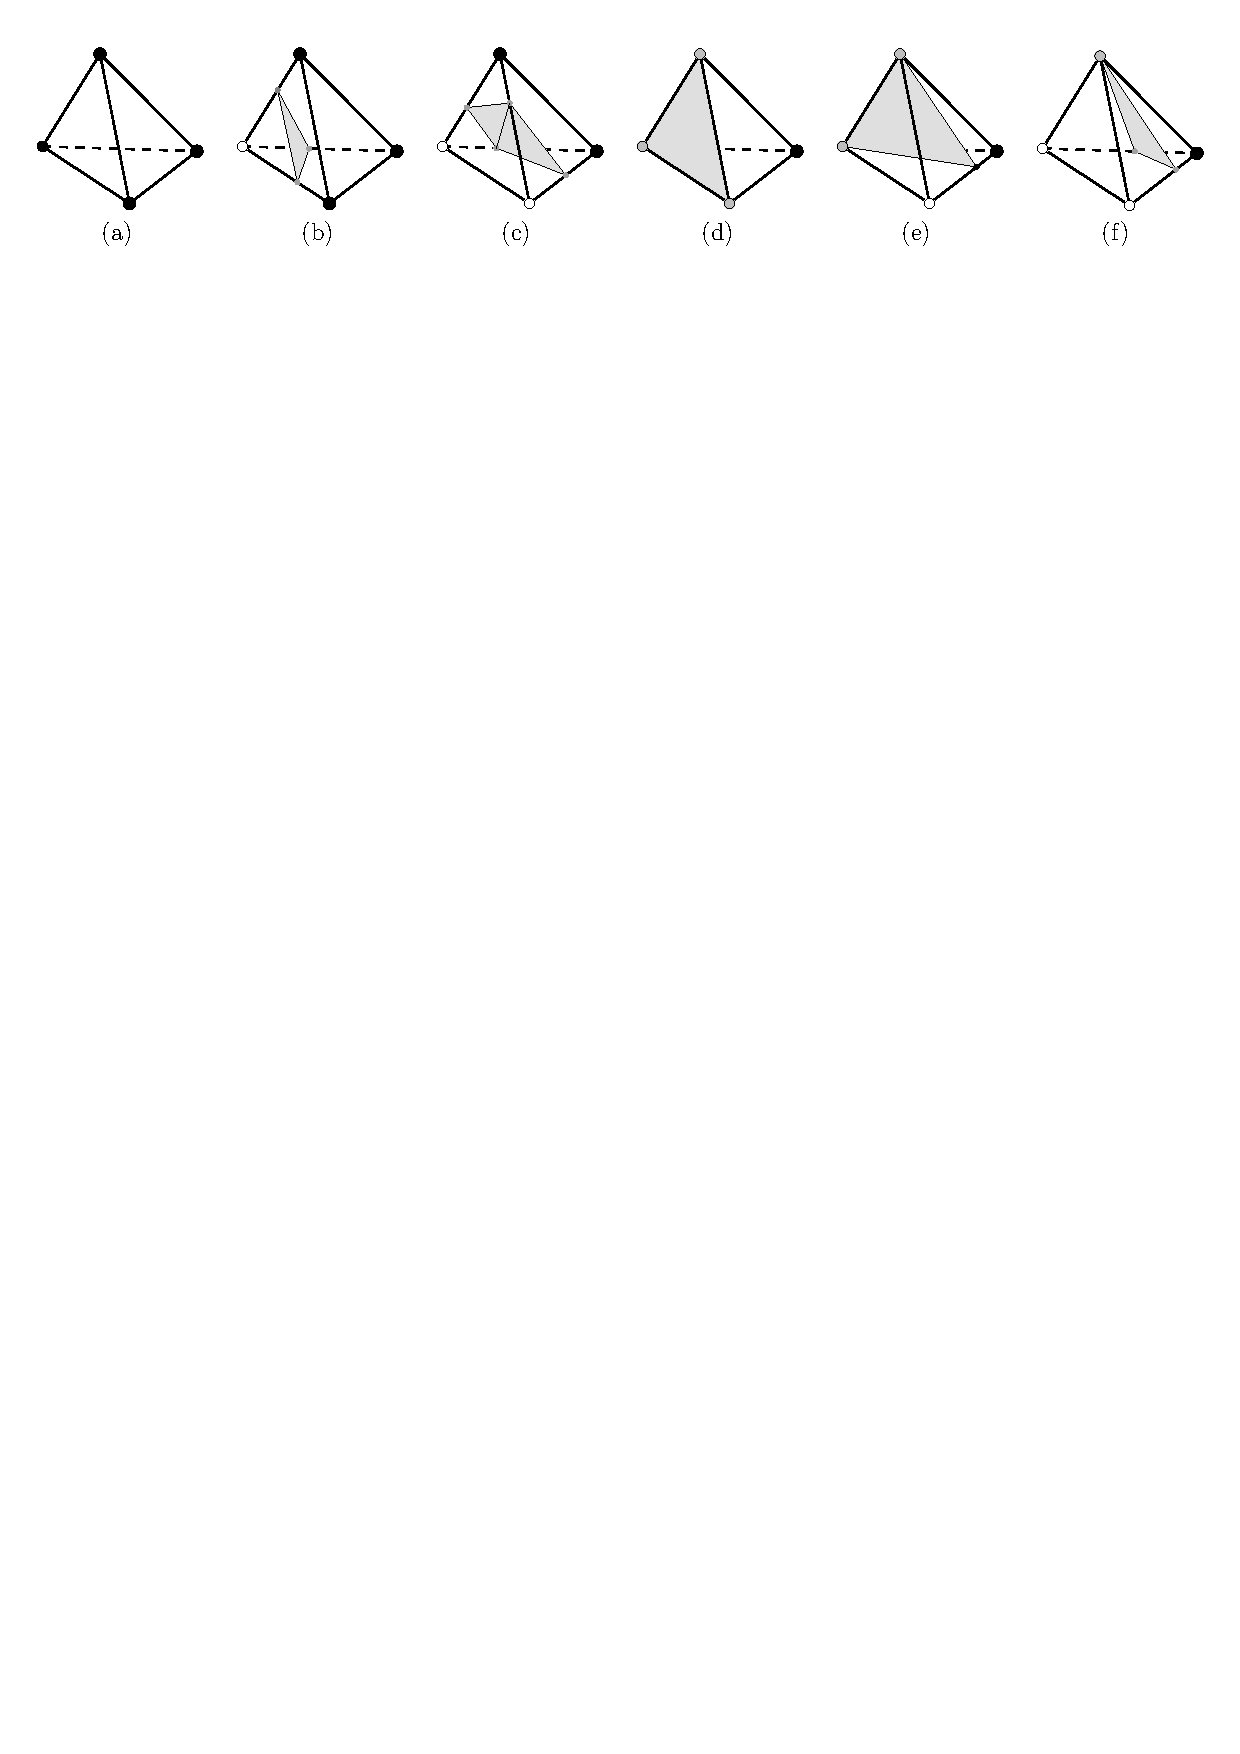
\includegraphics[width=1.0\textwidth]{figs/isosurface_3cases}
  \caption[Potential isosurface extracted for one tetrahedron]{Potential isosurface (for an attribute value $v$) extracted for one tetrahedron. Black vertex means that the attribute of this vertex is below $v$; white vertex means it is above; and grey that it is equal.}% 
\label{fig:isosurface_3cases}
\end{figure}
The only degenerate cases possible are when one or more vertices have exactly the same value as the isosurface. 
These cases are handled very easily, and the intersection is simply assumed to be at the vertices themselves (see Figure~\ref{fig:isosurface_3cases}d/e/f). 
Notice that the case when three vertices have exactly the same value, then the complete face of the tetrahedron must be extracted to ensure topological consistency.


%%%
%
\section[Adding constraints]{Constrained tetrahedralisations}%
\label{sec:cdt}

% p.95 of the delaunay book

As is the case in 2D, given as input a set of points, straight-line segments, and faces embedded in $\mathbb{R}^3$, two different Delaunay tetrahedralisations are possible:
\begin{itemize}
  \item conforming Delaunay tetrahedralisation (ConfDT)
  \item constrained Delaunay tetrahedralisation (ConsDT)
\end{itemize}
Both tetrahedralisations covers the convex hull of $\mathcal{P}$, respect every polygon (which can be represented by one or more triangles), and include every segment (which can be one of more edges in the tetrahedralisation) and vertex.

%

The typical input of a Delaunay tetrahedralisation program (or algorithm) is a called \emph{piecewise linear complex} (PLC).
Figure~\ref{fig:plc} shows one example.
\begin{marginfigure}
  \centering
  \includegraphics[width=0.95\linewidth]{figs/plc}
  \caption[A PLC representing a solid]{A PLC representing a solid (with a genus of 1) and having one dangling left; notice also that one extra edge is on a polygon. \textbf{Right:} These two polygons do not form a valid PLC because their intersection is not formed of vertices and edges in the PLC.}%
\label{fig:plc}
\end{marginfigure}
A PLC $\mathcal{P}$ is a set of linear $d$-cells (where $0 \leq d \leq 3$), that satisfy the following properties:
\begin{enumerate}
  \item the boundary of a $d$-cell in $\mathcal{P}$ is a union of cells in $\mathcal{P}$
  \item if two distinct cell $f, g \in \mathcal{P}$ intersect, their intersection is a union of cells in $\mathcal{P}$.
\end{enumerate}

As shown in Figure~\ref{fig:plc_not}, in practice this means that polygons cannot intersect other polygons (there needs to be a vertex and/or edges), but there are otherwise no restriction on the shapes that can be represented.
\begin{marginfigure}
  \centering
  \includegraphics[width=0.7\linewidth]{figs/plc_not}
  \caption[Two polygons that do not form a valid PLC]{These two polygons do not form a valid PLC because their intersection is not formed of vertices and edges in the PLC.}%
\label{fig:plc_not}
\end{marginfigure}
Observe also that a PLC is flexible and allows unconnected (\ie\ `floating') vertices, edges, and faces (an edge can for instance be inside a polygon).
Dangling edges, such as the one in Figure~\ref{fig:plc}, are also allowed.
The domain represented by a PLC does not have to represent a volume, it can be simply a set of points and surfaces that act as constraints for the tetrahedralisation.

%%%
\paragraph*{Tetrahedralisation of a polyhedron.}

If we use all the polygons bounding a polyhedron as the input PLC, the result is a tetrahedralisation of a polyhedron.
Figure~\ref{fig:meshing} shows one example, notice that the volume modelled by the boundary is tetrahedralised, but that here only some tetrahedra (in grey) are shown. 
\begin{figure}
  \centering
  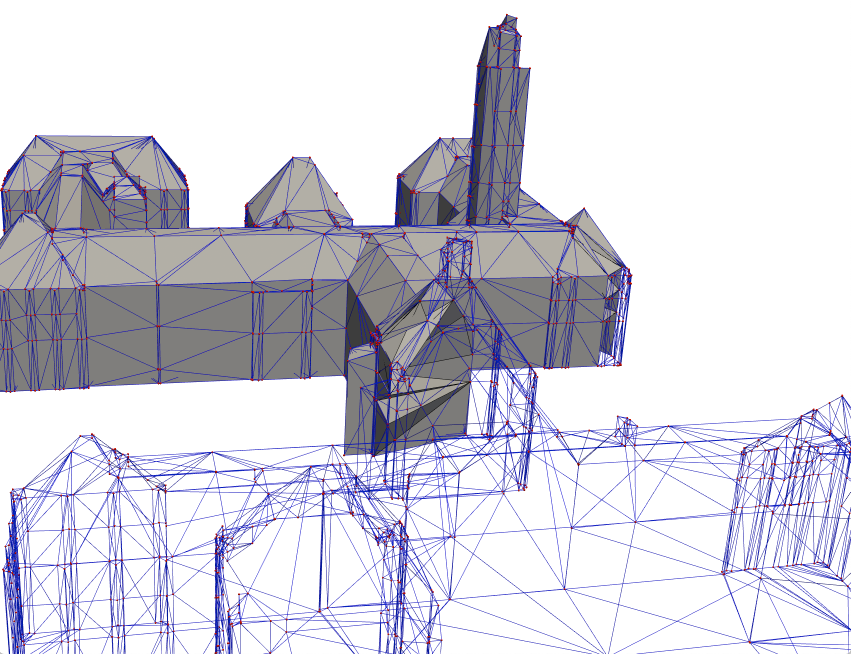
\includegraphics[width=\linewidth]{figs/mesh1}
  \caption{BK-City LoD2 b-rep tetrahedralised.}%
\label{fig:meshing}
\end{figure}
The surfaces of the b-rep also get meshed in the same process (each surface is triangulated).

While any polygon in two dimensions can be triangulated, some arbitrary polyhedra cannot be tetrahedralised without the addition of extra vertices, the so-called Steiner points. 
Figure~\ref{fig:schonhardt} shows a simple example, called the Sch\"onhardt polyhedron after the mathematician who first described the case.
\begin{marginfigure}
  \centering
  \includegraphics[width=0.95\textwidth]{figs/schonhardt}
  \caption[The Sch\"onhardt polyhedron]{The Sch\"onhardt polyhedron is impossible to tetrahedralise without adding extra vertices inside.}%
\label{fig:schonhardt}
\end{marginfigure}
This polyhedron is formed by twisting the top face of a triangular prism to form a 6-vertex polyhedron having eight triangular faces (each one of the three quadrilateral faces adjacent to the top face will fold into two triangles). 
It is impossible to select four vertices of the polyhedron such that a tetrahedron is totally contained inside the polyhedron, as none of the vertices of the bottom face can directly `see' the three vertices of the top triangular face.

%%%
\paragraph*{Conforming DT (ConfDT).}

A ConfDT is a tetrahedralisation where every tetrahedron has an empty circumsphere, it is thus a `real' Delaunay tetrahedralisation.   
This is achieved by adding new extra points to the input PLC $\mathcal{P}$ to ensure that the input constraints are present in the ConfDT\@. 
The extra points are called, as is the case in 2D, \emph{Steiner} points.
\marginnote{Steiner points}\index{Steiner points}

% 

It is known that every $n$-vertex PLC has a Steiner tetrahedralisation with at most $\mathcal{O}(n^2)$ vertices; notice here that this tetrahedralisation is \emph{not} necessarily Delaunay.

Obtaining a ConfDT might require inserting significantly more than this, when for instance two or more polygons form a very small angle.

In fact, there is no algorithm that can guarantee a polynomial number of vertices.

Most implementations will insert several new vertices, which are often unnecessary.
Because of this, ConfDT are less used in practice.


% There are algorithms that can find a Steiner Delaunay tetrahedralisation of any three-dimensional polyhedron, but they might introduce a superpolynomial number of new vertices. 
% No known algorithm for finding Steiner Delaunay tetrahedraliza- tions is guaranteed to introduce only a polynomial number of new vertices, and no algo- rithm of any complexity has been offered for four- or higher-dimensional Steiner Delaunay triangulations. 
% Moreover, the existing algorithms all seem to introduce an unnecessarily large number of vertices near small domain angles. These problems can be partly remedi- ated by Steiner CDTs.

% As Figures~\ref{fig:ccdt} and ~\ref{fig:cdt_example}c show, the input straight-line segments will be split into several collinear segments. 
% The Steiner points have to be carefully chosen (where to put them is beyond the scope of this course).
% Observe that each triangle in a ConfDT respect the Delaunay criterion, but that more triangles are present. 
% If 2 segments are nearly parallel, many points could be necessary (for $m$ segments, up to $m^2$ could be necessary).



%%%
%
\paragraph*{Constrained DT (ConsDT).}

Given a PLC $\mathcal{P}$, the ConsDT is similar to the Delaunay tetrahedralisation, but the tetrahedra in ConsDT are not necessarily Delaunay (\ie\ their circumsphere might contain other points from $\mathcal{P}$). 
The empty circumsphere for a ConsDT is less strict: a tetrahedron is Delaunay if its circumsphere contains no other points in $\mathcal{P}$ that are \emph{visible} from the tetrahedron; the constraints polygons in $\mathcal{P}$ act a visibility blockers. 

%

Thus, the ConsDT aims at keeping the Delaunay properties, but relaxes them to be able to respect the constraints (edges and polygons in the PLC).
% \begin{figure*}
%   \centering
%   \includegraphics[width=0.95\linewidth]{figs/cdt_tudelft}
%   \caption[A ConsDT of each building of the TU Delft]{The LoD1 3D model of the TU Delft where each building is represented with the ConsDT of its PLC.}%
% \label{fig:cdt_tudelft}
% \end{figure*}

%

However, unlike in 2D where it is known that for a set $S$ of points and straight-line segments there is always a ConsDT possible, in 3D this is not the case.
As explained above, this is linking to the fact that simple PLC cannot be tetrahedralised at all.
As a consequence, the ConsDT of a PLC in 3D allows extra Steiner vertices to be inserted.
The existing algorithms (and their implementations) that will insert far fewer vertices in a ConsDT than in a ConfDT\@. 
The details of the algorithms are beyond what is covered in this course.

%

\newpage
\begin{kaobox}[frametitle=\faCog\ How does it work in practice?]
  Implementing a ConsDT that is robust against all input is difficult, and there exists few reliable libraries.
  Perhaps the ``best'' and easiest to use is TetGen, which is open-source; it is available at \url{http://www.tetgen.org/}.
  Beware: it expects a \emph{perfect} input PLC, which is often not available for 3D geographical datasets that are made available by municipalities and governments; see Chapter~\ref{chap:iso19107}.
\end{kaobox}


%%%
%
\section{Notes and comments}
% TODO : complete notes

\citet{Rajan91} shows that the smallest sphere containing a Delaunay tetrahedron is smaller than the one of any other tetrahedron, \ie\ the Delaunay criterion favours `round' tetrahedra.

\citet{Cignoni98} developed an algorithm, called \texttt{DeWall} and based on the divide-and-conquer paradigm, for constructing the DT in any dimensions. Although the worst-time complexity of this algorithm is $\mathcal{O}(n^3)$ in three dimensions, they affirm that the speed of their implementation is comparable to the implementation of known incremental algorithms, and is sub-quadratic.

The Schönhardt polyhedron was first described in \citet{Schonhardt28}. 

The algorithm to construct the 3D DT is adapted from~\cite{Joe91}, and is conceptually the same as~\cite{Edelsbrunner96}. 
See \citet{Ledoux07} for an easy explanation of the steps to construct the 3D DT/VD for a set of points, including the handling of the degeneracies. 

\citet{Ledoux08} presents an overview of why the VD is a better alternatives to grids for the modelling of geoscientific fields.

\citet{Cheng00} and \citet{Miller02} both describe methods to remove slivers in Delaunay meshes and to improve the shape of tetrahedra (so that they can be used for interpolation).

%%%
%
\section{Exercises}

\begin{enumerate}
  \item A DT contains 32 tetrahedra and we insert a new point $p$ that falls inside one of the tetrahedra. If we insert and update the tetrahedralisation (for the Delaunay criterion), what is the number of tetrahedra?
  \item If a given vertex $v$ in a DT has 18 incident tetrahedra, how many vertices will its dual Voronoi cell contain?
  \item Take a cube and try tetrahedralise it (not necessarily into Delaunay tetrahedra). How many tetrahedra do you get?
  \item If $a = (1, 1, 2)$, $b = (4, 2, 2)$, $c = (3, 3, 2)$, and $d = (4, 3, 3)$. Is the value returned by \Orient~($a,b,c,d$) positive, negative, or 0?  
\end{enumerate}
